\part{Nový pozorovatelný příznak svazků}


%Cílem experimentu je objevit další parametr světelného svazku, jenž by v kombinaci s ostatními parametry pomohl rozpoznat měřené svazky. 

\section{Vzájemná rotace kamene a zdrojového svazku}
Pokusíme se nalézt směr či velikost rotace světelných svazků při rotaci kamene nebo při naklonění zdroje dopadajícího světelného svazku. 

Rotace kamene kolem osy způsobí změnu vlastností vystupujících světelných svazků (směru, zářivého toku, intenzity, vlastnosti ocásků atd.). Za určitých okolností může světelný svazek zcela vymizet. Tato situace nastává například při lomu světelného svazku z kamene do okolí. Když vlivem rotace překročíme kritický úhel, nedochází k lomu světelného svazku, ale k totálnímu odrazu na fasetě. Světelný svazek zanikne při posunu světelného svazku mimo fasetu, a to jak při odrazu, tak při lomu. Ze stejných důvodů, proč mohou světelné svazky vymizet, mohou naopak vzniknout svazky nové.

Uvažujeme zjednodušenou situaci, kdy světelný svazek nahradíme světelným paprskem ležícím v jeho pomyslném těžišti. 

Světelný paprsek necháme dopadat na zrcadlo pod úhlem $\varphi_1$. Paprsek se od zrcadla odráží podle známého zákonu odrazu pod úhlem $\varphi_1$. Při vychýlení světelného paprsku o úhel $ \delta $ v~ kladném směru úhlu $\varphi_1$ je odražený úhel $\varphi_1 + \delta$. Úhel odraženého paprsek se změní o úhel $ \delta $.

\begin{figure}[h!]
\begin{center}
\scalebox{1}{ \input{xfig/odraz2.pstex_t}}
\end{center}
\caption[Odraz světelného paprsku od zrcadla.]{Odraz světelného paprsku od zrcadla. Změna úhlu dopadajícího světelného paprsku vyvolá stejně velkou změnu úhlu odraženého paprsku.}
\label{fig:odraz laser}
\end{figure}

Jiná situace nastává při rotaci zrcadla kolem osy o úhel $\alpha$ v záporném směru. Světelný paprsek dopadá na zrcadlo pod úhlem $\varphi_1 + \alpha$ a  odráží se pod úhlem $\varphi_1+\alpha$. Úhel odraženého paprsku se v tomto případě změní o úhel $2\alpha$. 

Při rotaci kamene docílíme stejné změny odraženého paprsku jako při rotaci světelného zdroje o dvojnásobný úhel v opačném směru. Proto budeme dále uvažovat pouze rotaci kamene. 


\begin{figure}[h!]
\begin{center}
\scalebox{1}{ \input{xfig/odraz.pstex_t}}
\end{center}
\caption[Odraz světelného paprsku od rotujícího zrcadla.]{Odraz světelného paprsku od rotujícího zrcadla. Rotace zrcadla vyvolá dvojnásobnou změnu velikosti úhlu odraženého paprsku.}
\label{fig:odraz zrcadlo}
\end{figure}

\section{Změna směru vystupujících paprsků}
\label{sec: zmena smeru}
Pokud by docházelo pouze k odrazu od zrcadel v dvojrozměrné rovině, tak by naše zkoumání postrádalo smysl. Výstupní parsek by se vždy otočil o dvojnásobek úhlu rotace kamene, a to ve stejném směru. 

S uvažováním materiálu kamene s konstantním indexem lomu $ n_1~>~1 $ a okolí s indexem lomu $ n_2 = 1 $ se situace dramaticky mění. Vezměme si příklad lomu světelného paprsku z kamene přes rovinnou fasetu. Úhel dopadajícího paprsku na fasetu označme $\alpha_1$ a úhel lomeného svazku $\alpha_2$, pak můžeme podle Snellova zákona psát:

\begin{center}
$n_1\,\sin(\alpha_1) = n_2\,\sin(\alpha_2) = \sin(\alpha_2)\,.$
\end{center}

\begin{figure}[h!]
\begin{center}
\scalebox{.9}{ \input{xfig/index.pstex_t}}
\end{center}
\caption[Kritický úhel a totální odraz.]{Tři případy, které mohou nastat při dopadu světelného paprsku na fasetu. Zleva lom paprsku z kamene, dopad pod kritickým úhlem a totální odraz.}
\label{fig:lom ven }
\end{figure}

Zkoumejme změnu výstupního úhlu $\alpha_2$ na změně úhlu $\alpha_1$. Nejprve si vyjádříme úhel $\alpha_2$ následně zderivujeme podle $\alpha_1$. 
\begin{equation}
\alpha_2 = \arcsin(n_1\,\sin\alpha_1)
\label{eq:derivace uhlu1}  
\end{equation}
\begin{equation} \frac{\mathrm{d}\alpha_2}{\mathrm{d}\alpha_1}= \frac{n_1\,\cos\alpha_1}{\sqrt{1-n_1^2\,\sin^2\alpha_1}}
\label{eq:derivace uhlu}  
\end{equation}

Pokud se dostáváme ke kritickému úhlu ($\alpha_1 = \alpha_k$), dochází k totálnímu odrazu. 
\begin{equation}
 \sin\alpha_2 = 1 \implies \sin\alpha_1 = \frac{1}{n_1}
\end{equation}

Výpočtem limity rovnice \ref{eq:derivace uhlu} v okolí kritického úhlu pro $ n_1 > 1$ dostaneme 

\begin{eqnarray}
\lim_{\alpha_1 \to \alpha_k}\frac{\mathrm{d}\alpha_2}{\mathrm{d}\alpha_1} = \frac{n_1\,\cos(\arcsin\frac{1}{n_1})}{\sqrt{1-n_1^2\,\frac{1}{n_1^2}}} \to \infty\,.
\label{eq:zmena velikosti posunu}  
\end{eqnarray},

Z grafu \ref{fig:derivace uhlu} zjistíme, že minimum funkce $\frac{\mathrm{d}\alpha_2}{\mathrm{d}\alpha_1}$ vychází pro $ \alpha_1 = 0^\circ $. Po dosazení
\begin{eqnarray}
{\frac{\mathrm{d}\alpha_2}{\mathrm{d}\alpha_1}}\biggr\rvert_{\alpha_1 = 0^\circ}= \frac{n_1}{\sqrt{1-0}} = n_1\,.
\end{eqnarray}


Velikost změny posunu světelného svazku tedy může být teoreticky libovolně větší než je index lomu $n_1$. 

\begin{figure}[h!]
\begin{center}
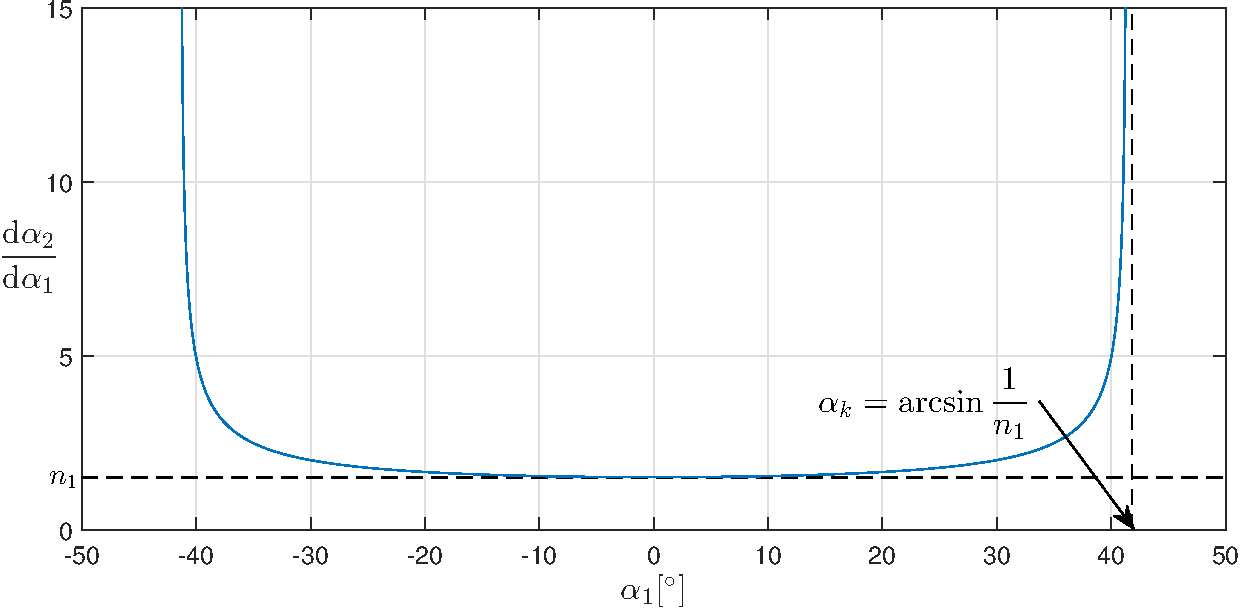
\includegraphics[width = 0.8\linewidth]{derivace.pdf}
\end{center}
\caption[Závislost změny lomeného úhlu na změně úhlu dopadu.]{Závislost změny lomeného úhlu na změně úhlu dopadu. Pro kritický úhel $\alpha_k$ roste k~nekonečnu. Graf funkce popsané vzorcem \ref{eq:zmena velikosti posunu}.}
\label{fig:derivace uhlu}
\end{figure}



\section{Modelování pohybu svazků}
V programu LADOK jsme provedli experiment s rotací broušeného kamene \textit{viva12}.

Rotací kamene okolo osy kolmé ke spodku kamene dostaneme pouze soustředné kružnice. Kámen jsme tedy rotovali kolem vodorovné osy procházející středem spodku kamene o konstantní úhel v každém kroku. Zaznamenali jsme směry vystupujících svazků při různých pozicích kamene. Výsledek jsme vykreslili do polárního grafu. Ze dvou po sobě následujících pozic kamene jsme šipkou spojili pozici svazků se stejným seznamem dopadových faset. Výsledný obrazec je znázorněn na obr. \ref{fig:relativni pohyb graf}.

Z praktického hlediska nás mohou zajímat pouze svazky, které vytvoří po dopadu na stínítko detekovatelnou stoupu.

% obrazek pohybu jednotlivych stop 
\begin{figure}[h!]
\begin{center}
   \begin{minipage}[c]{0.48\textwidth}
     \centering 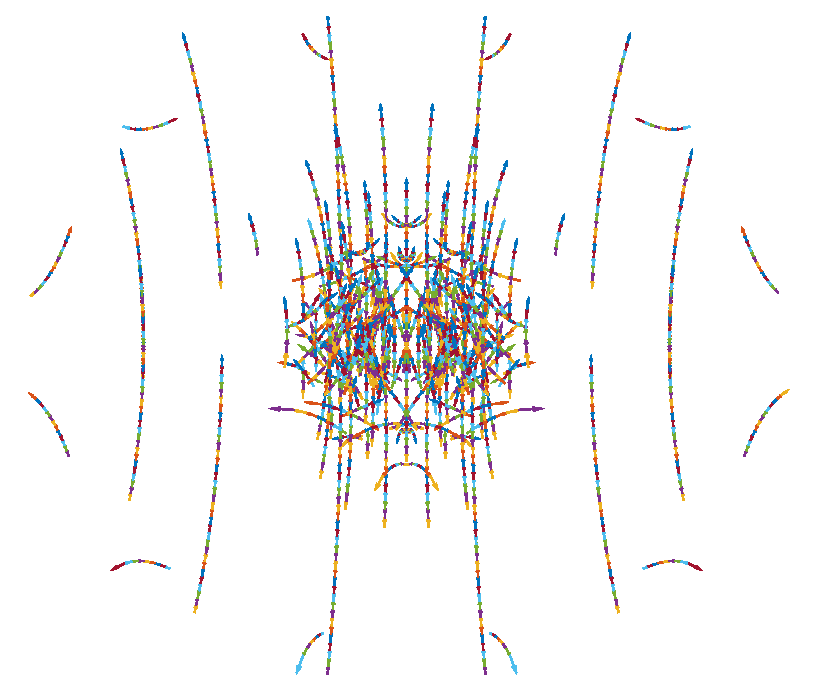
\includegraphics[width = 1\linewidth]{viva12_bigflux.eps}
   \end{minipage}
   \begin{minipage}[c]{0.48\textwidth}
     \centering 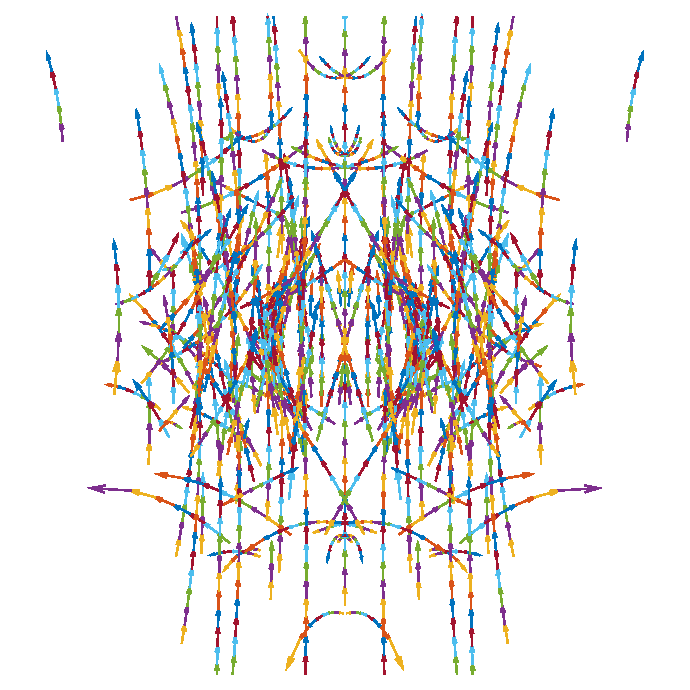
\includegraphics[width = 1\linewidth]{viva12_bigflux2.eps}
   \end{minipage}
 \end{center}
\caption[Dráhy pohybu svazků při rotaci kamene.]{Dráhy směru svazků vycházejících z kamene \textit{viva12} získané pomocí simulačního programu  LADOK při rotaci kamene. Zobrazeny jsou pouze svazky s významným zářivým tokem vycházející v horního poloprostoru kamene. Vpravo detail na střed obrázku vlevo.}

\label{fig:relativni pohyb graf}
\end{figure}

Pro lepší představu o změně směru jednotlivých svazků nám může být užitečný kruhový histogram znázorňující směr jejich pohybu (obr. \ref{fig:relativni pohyb graf}). Podstatná většina svazků se posouvá ve směru rotace kamene, což není příliš nápomocné při jejich identifikaci.

Existují však svazky, které jsou svým pohybem charakteristické a lze je tedy oddělit od ostatních. Kritérium pro rozpoznání svazků nemusí být pouze směr pohybu, ale jak vidíme na obr. \ref{fig:relativni pohyb graf} i velikost úhlu rotace. V neposlední řadě přichází v úvahu i změna zářivého toku svazků, změna velikosti ocásků a další. 

\begin{figure}[h!]
 \begin{center}
   \begin{minipage}[c]{0.48\textwidth}
     \centering 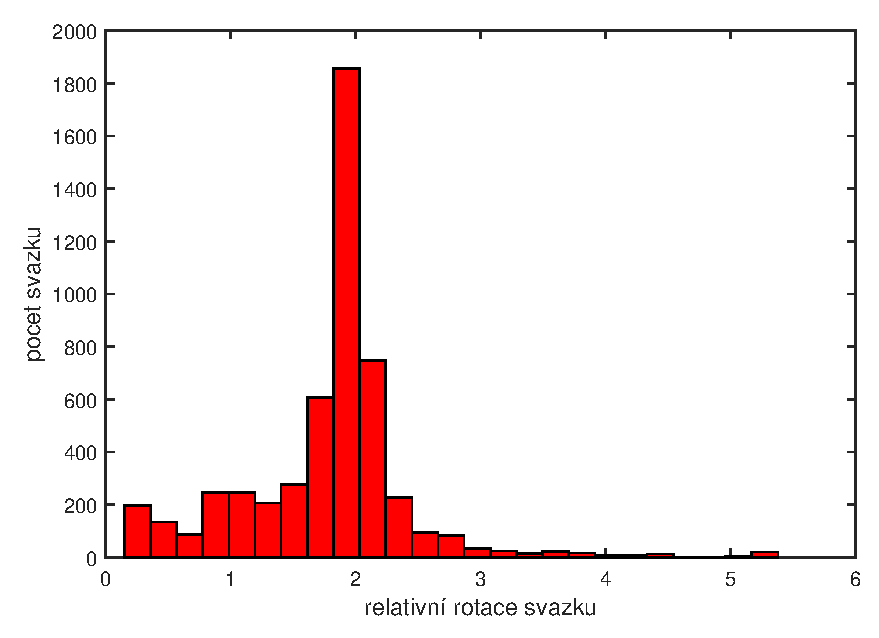
\includegraphics[width = \linewidth]{relative.eps} 
   \end{minipage}
   \begin{minipage}[c]{0.48\textwidth}
     \centering 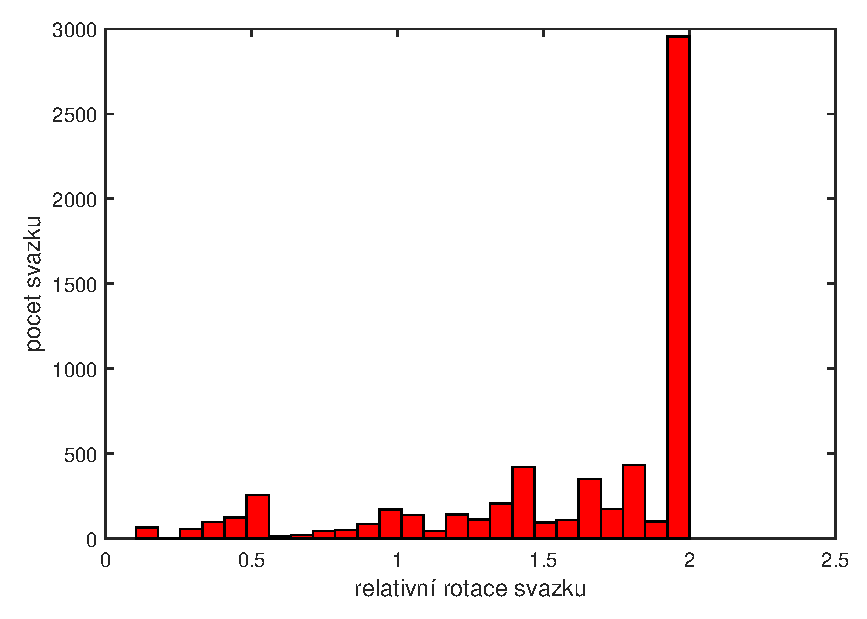
\includegraphics[width =\linewidth]{relative_index1.eps} 
   \end{minipage}
 \end{center}
\caption[Histogram velikosti rotace vystupujících svazků.]{Vlevo: histogram velikosti úhlu rotace vystupujících svazků z kamene \textit{viva12} z obrázku \ref{fig:relativni pohyb graf}. Vlivem lomu je relativní rotace v mnoha případech větší než 2. V okolí kritického úhlu roste k~nekonečnu. Pokud ztotožníme indexy lomu kamene a okolí, tak relativní rotace nebude větší než 2. To lze vidět na histogramu vpravo.}

\label{fig:histogram relativni pohyb }

\end{figure}

Vykresleme si histogram (obr. \ref{fig:histogram relativni pohyb } vlevo) relativní velikosti úhlu rotace vystupujících svazků. Z něj je patrné, že řada svazků rotuje o více než dvojnásobek úhlu rotace kamene $\alpha$, což potvrzuje teorii o relativní změně směru svazků z rovnice \ref{eq:zmena velikosti posunu}. 



\begin{figure}[h!]
\begin{center}
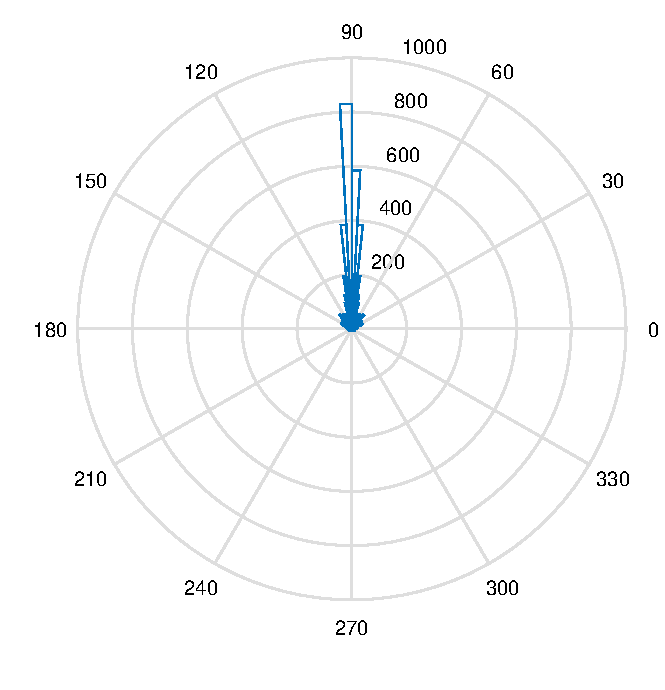
\includegraphics[width =0.7\linewidth]{kruhovy_histogram.eps}
\end{center}
\caption[Kruhový histogram směru rotace svazků - \textit{viva12}.]{Kruhový histogram směru rotace vystupujících svazků kamene \textit{viva12} z obrázku \ref{fig:relativni pohyb graf}. Většina svazků se pohybuje ve směru rotace kamene.}
\label{fig:kruhovy histogram}
\end{figure}

Pokud vezmeme kámen o stejném indexu lomu, jako je okolí, nedochází k lomu. Potom by se nemělo docházet k rotaci výstupního svazku o úhel větší než $2\alpha$, způsobená právě rozdílným indexem lomu. Pro potvrzení této teorie jsme provedli stejnou simulaci jako v~předchozím případě. Indexy lomu kamene a jeho okolí jsme ztotožnili a výsledek simulace ukázal, že rotace výstupních svazků úhel větší než $2\alpha$ se již nevyskytují. To nám dokládá zhotovený histogram (obr. \ref{fig:histogram relativni pohyb } vpravo).


Téměř konstantní směrovost rotace svazků u kamene \textit{viva12} zmenšuje význam příspěvku této vlastnosti k lepšímu rozpoznání světelných stop. Pokud ovšem provedeme stejný experiment na broušeném kameni jiného tvaru, dostaneme rozdílný výsledek. Například u šatonu, svým tvarem složitějším než \textit{viva12}, je směr rotace svazků rozmanitější. Velká část z nich samozřejmě rotuje ve směru rotace kamene. Jak ale vidíme z kruhového histogramu (obr. \ref{fig:kruhovy histogram saton}), lze rozlišovat i velké množství stop pohybujících se např. pod úhlem $45^\circ$. U šatonu tedy může znalost směru pohybu svazků při rotaci kamene nemalou měrou pomoci v jejich rozpoznání. 

\begin{figure}
\begin{center}
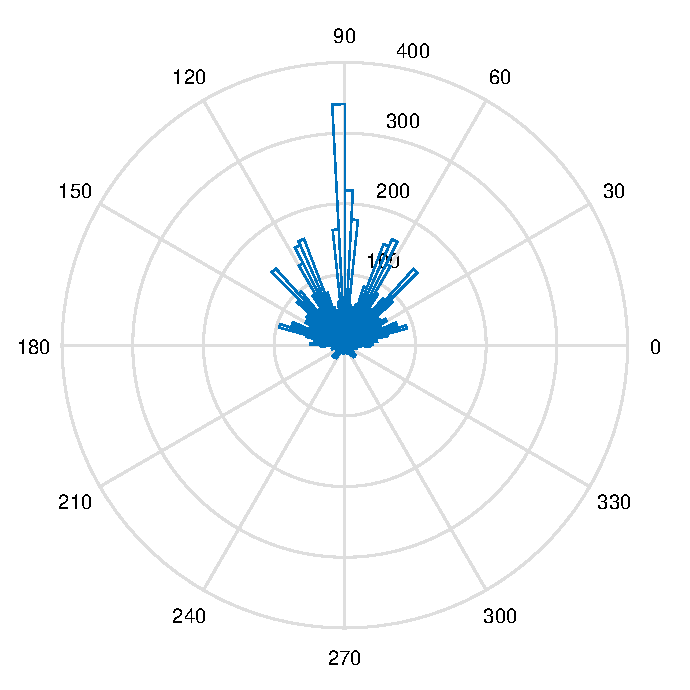
\includegraphics[width = 0.7\textwidth]{saton_smer.eps}
\end{center}
\caption[Kruhový histogram směru rotace svazků - šaton.]{Kruhový histogram směru rotace vystupujících svazků z šatonu při rotaci kamene.}

\label{fig:kruhovy histogram saton}
\end{figure}

  
\clearpage